\documentclass[]{amsart}
\usepackage{hyperref}
\usepackage{listings}
\usepackage{graphicx}  % include graphics
\usepackage{subfig}       % multiple figures in a graphics plot
\lstset{language=Python}

\begin{document}

\title{SpaceX Data Science Write-up}
\author{Paul Gribelyuk}
\date{Today}
\maketitle

\textbf{Estimating the Quality of Shuttle Valves}

The approach I took was to estimate the distribution of each time-series.  Specifically, I model each point in the time-series as a single-parameter Gaussian, $y\sim\mathcal{N}(\theta, \sigma)$ with that parameter having a Gaussian distribution $\theta\sim\mathcal{N}(\mu, \tau)$.  I then if a new data-point $y_1$ arrives, the updates is as follows:
\begin{eqnarray*}
\mu_1 &=& \frac{\frac{1}{\tau_0}\mu_0 + \frac{1}{\sigma^2}y_1}{\frac{1}{\tau^2_0} + \frac{1}{\sigma^2}} \\
\frac{1}{\tau^2_1} &=& \frac{1}{\tau^2_0} + \frac{1}{\sigma^2}
\end{eqnarray*}
Since, there are 1000 data points in each time-series, I create a chain of 999 nodes (the first one is left off, since $y$ models the differences and not the values themselves), and update it 4 times.  To perform inference and estimate whether an input time-series is good or bad, I implemented a log-likelihood function:
$$
\mathcal{L}(\mathbb{Y}|\theta) = \sum\log\{p(y_i|\theta)\}
$$
The determination is made based on which model produces a higher log-likelihood.  Some of the class which I implemented to help with these Bayesian updates are:
\begin{itemize}
\item \verb|SingleParamNormal|: this class handles the updating; takes an initial value for the $\mu$, $\tau$, and $\sigma$
\item \verb|NormalChain|: creates a chain of normals, updates constituent Gaussian nodes, and can generate the log-likelihood for a new series
\item \verb|Predictor|: initialized with some NormalChain objects, and can make a prediction of how to classify a new time-series
\end{itemize}

All the code is in the included \verb|valve.py| as well as the iPython Notebook (althought that is strictly for experimentaiton.\\
\\
Results\\
The model was primitive as only 1 parameter, the mean, was being learned.  Even so, it is able to classify the two types series, even when leaving one series out of the training (as detailed in the \verb|__main__|).  Here is sample output:
\begin{verbatim}
paul$ python3 valve.py
good series
good good good good
bad series:  bad bad bad bad bad bad bad bad
\end{verbatim}

A next step would be to create a two-parameter learner which also learns the $\theta_2 = \sigma$.\\

The learned path (taking 1000 simulations) looks as follows:
\begin{figure}[ht!]
  \centering
    \subfloat{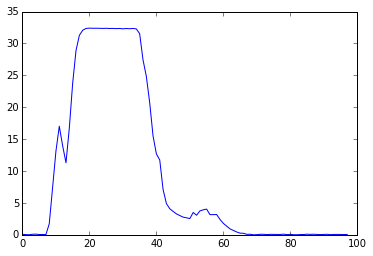
\includegraphics[width=0.45\linewidth]{good_path.png}}
    \subfloat{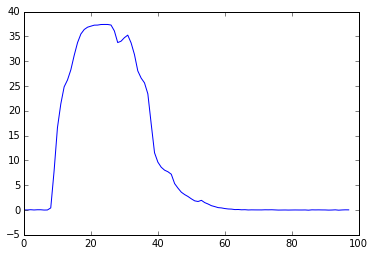
\includegraphics[width=0.45\linewidth]{bad_path.png}} \\
  \caption{Learned Good (left) and Bad Paths}
\end{figure}


\end{document}